\subsection{Discretización de datos numéricos}

\textbf{Descripción:} La discretización consistió en convertir atributos numéricos en categóricos, las estrategias
de discretización que se utilizaron fueron: por frecuencia (generan bins en cantidades similares de instancias en cada uno),  densidad
(con bins del mismo ancho), y supervisado (utiliza un modelo de discretización que toma en cuenta la clase en
el armado de los bins) 

\textbf{Metodología utilizada:} para este experimento, se crearon conjuntos de datos para cada
una de las tres estrategias de discretización previamente comentadas, para crear los bins por frecuencia
y densidad se utilizo la biblioteca 'arules', y para la discretización supervisada
se uso la biblioteca 'RWeka'.  

Para la discretización por frecuencia y densidad se varió la cantidad de bins entre 1 y 20.
Cabe resaltar que elegir 1 bin implica prescindir del atributo discretizado a la hora de
construir el árbol, ya que el mismo tomaría un solo valor.

Para la discretización supervisada, no es posible seleccionar la cantidad de bins de salida
ya que la misma es determinada por el propio filtro utilizando un criterio de entropía sobre
ganancia de información.

Se hicieron corridas sobre las tres familias utilizando el algoritmo J48 variando el CF de
forma análoga a lo hecho en la Sección II.

Con las salidas, se analizó, para los casos de discretización no supervisada, la relación
entre la cantidad de bins, la cantidad de nodos del árbol de clasificación y su performance.
Asimismo, se compararon las distintas estrategias entre sí, y contra los resultados de la
Sección II.

\textbf{Análisis de los resultados:} Los resultados obtenidos una vez realizado el experimento
se pueden resumir en las figuras presentadas a continuación.

La figura~\ref{fig:overdis}, hace referencia a la discretización supervisada, se puede
dar cuenta que son muy similares a la figuras de sobreajuste y poda sin discretización.


\begin{figure*}
  \centering
  \subfigure[Leaves vs CF]{\label{b1} 
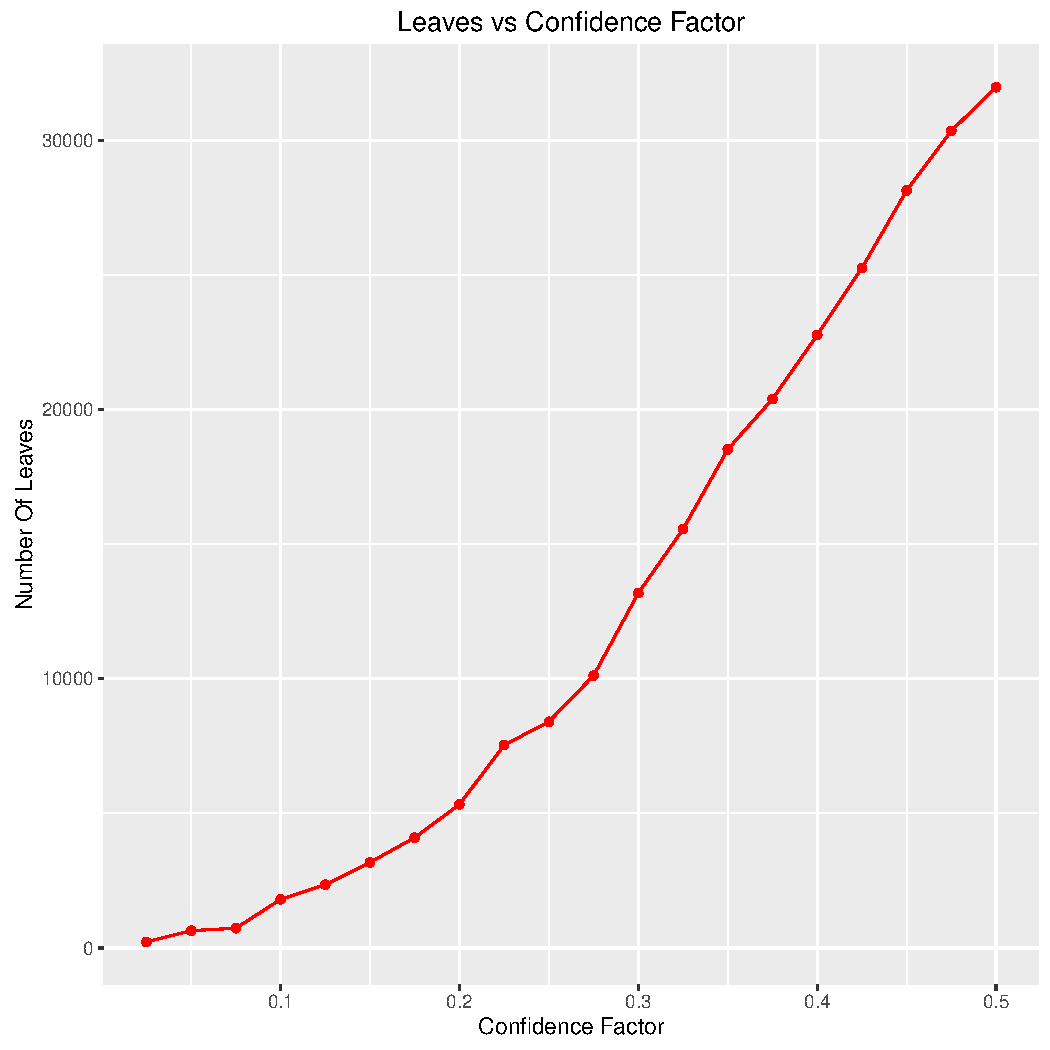
\includegraphics[width = 7cm]{6a.pdf}}
  \subfigure[Accuracy vs CF]{\label{b2}
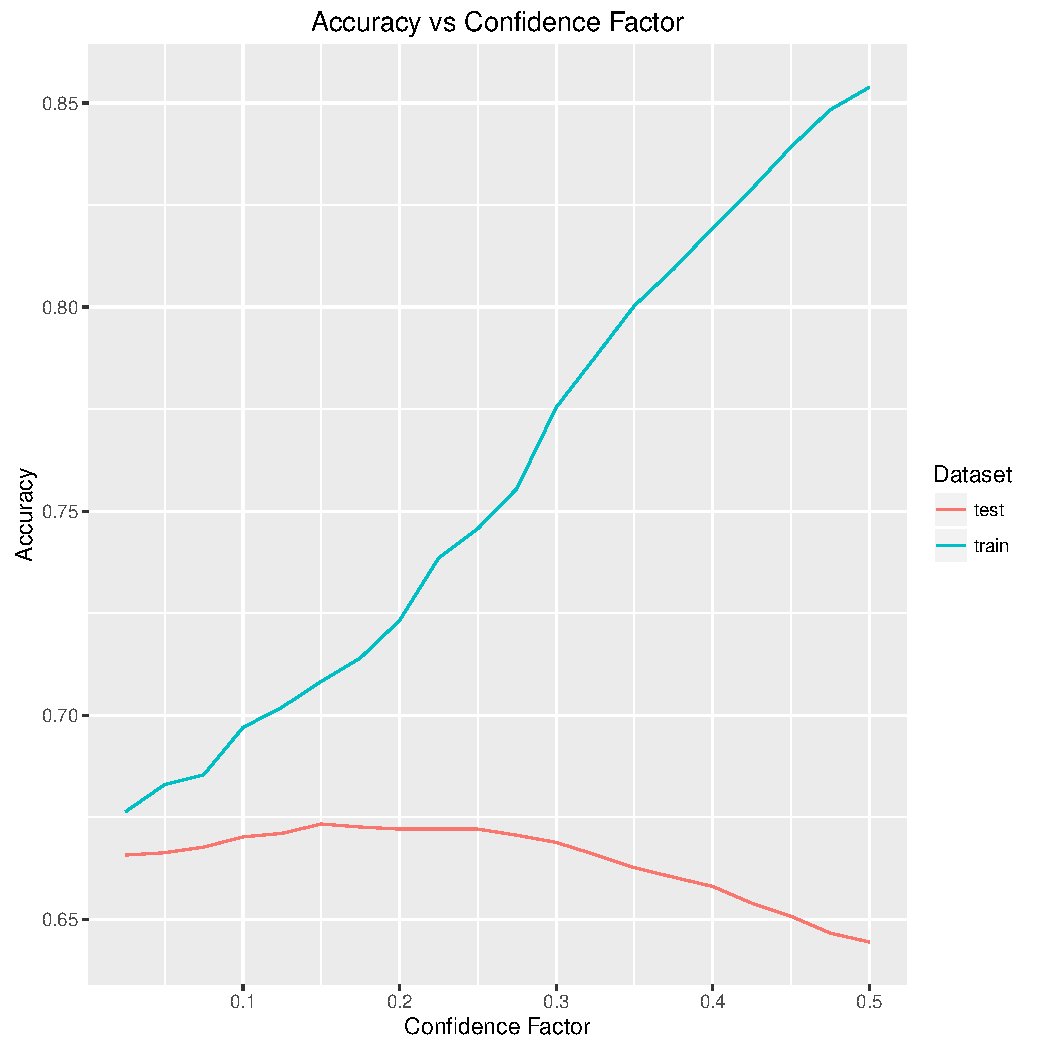
\includegraphics[width = 7cm]{6b.pdf}}
    \subfigure[ROC curve better tree]{\label{b3}
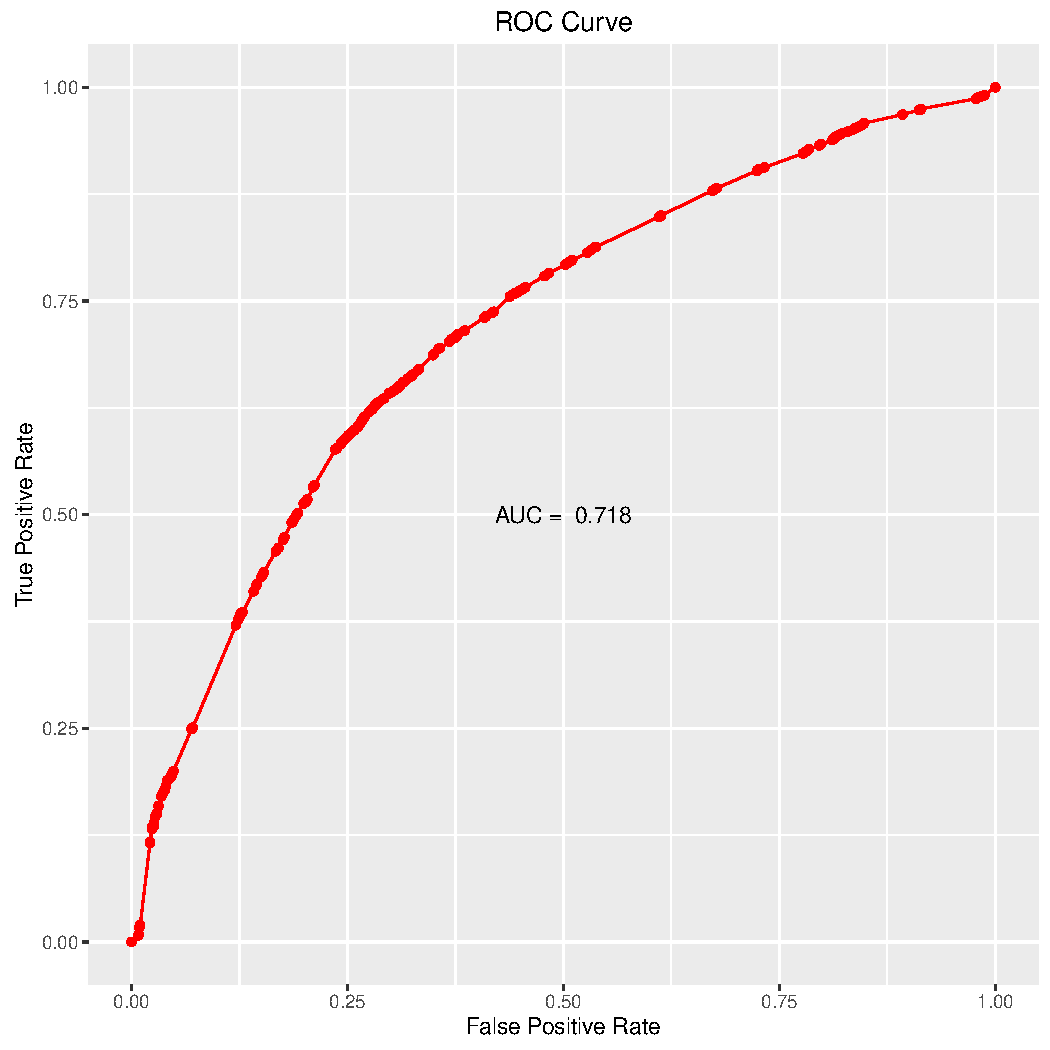
\includegraphics[width = 7cm]{6c.pdf}}
  \caption{overfitting and pruning discretize}
  \label{fig:overdis}
\end{figure*}


En la figura~\ref{fig:6d} se observa que hay un nivel de asociación positivo entre los bins
utilizados en la estrategia de discretización y los nodos del árbol de clasificación, en línea
con lo esperado. Las líneas, que representan la estrategia empleada se cruzan en varios
tramos de la representación, lo que no permite determinar si la asociación enunciada es
más fuerte en una o en otra.

\begin{figure}
  \centering
  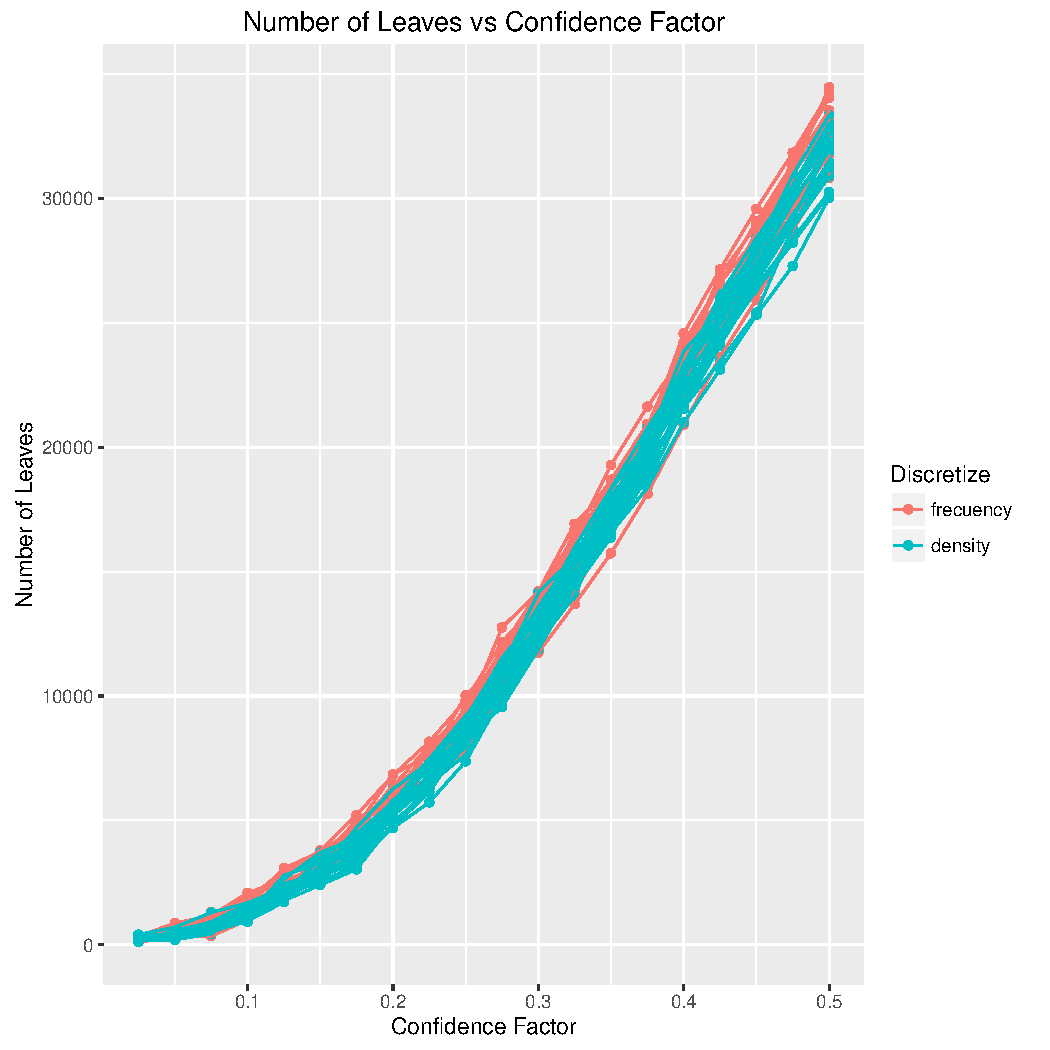
\includegraphics[width = 8cm]{6d.pdf}
  \caption{Leaves vs missing percentage with discretize}
  \label{fig:6d}
\end{figure}

En la figura~\ref{fig:discretize} muetran la precisión del árbol en función del CF para la discretización
por frecuencia y densidad respectivamente, se observa que las precisiones se encuentran en la discretización
por densidad pero la diferencia es muy mínima.


\begin{figure*}
  \centering
  \subfigure[Frequency discretize]{\label{b1} 
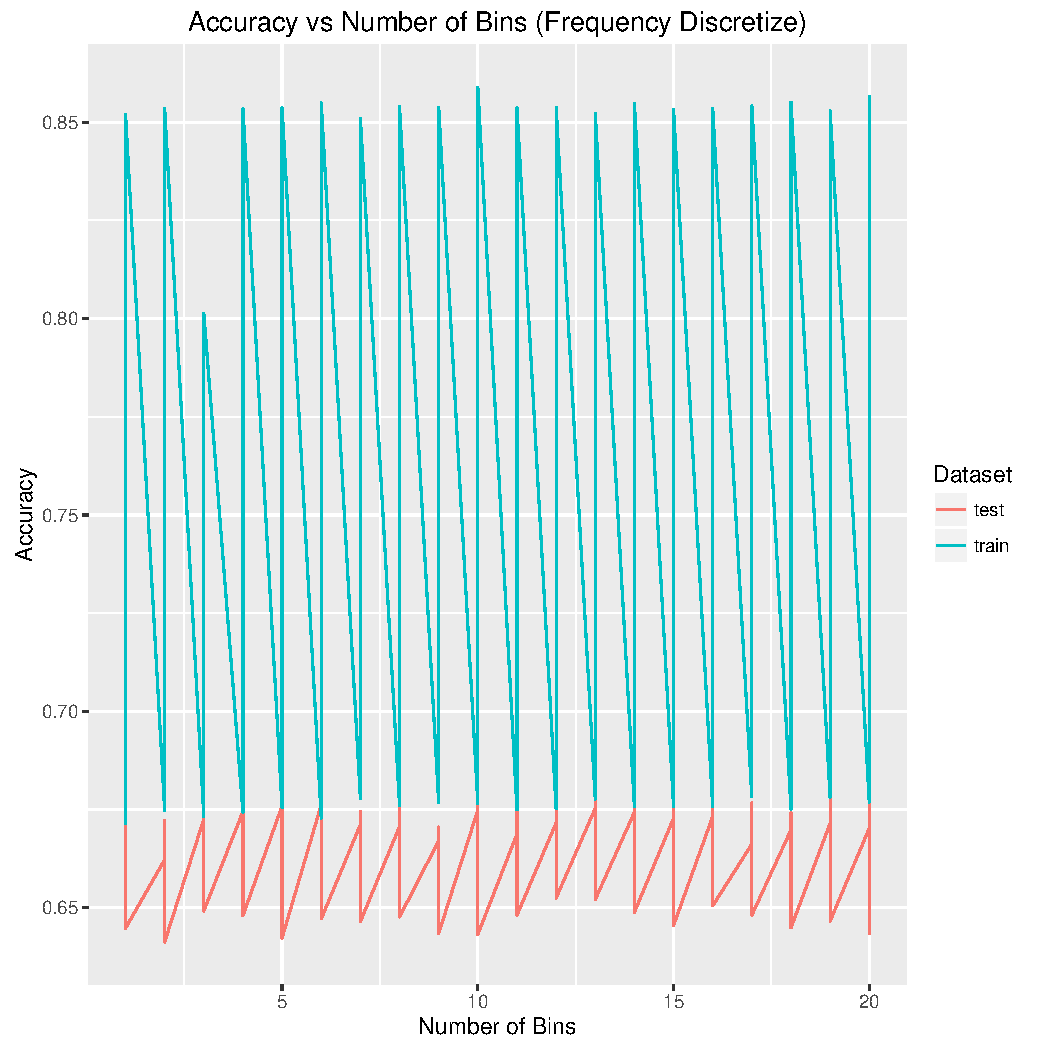
\includegraphics[width = 7cm]{6e.pdf}}
  \subfigure[Density discretize]{\label{b2}
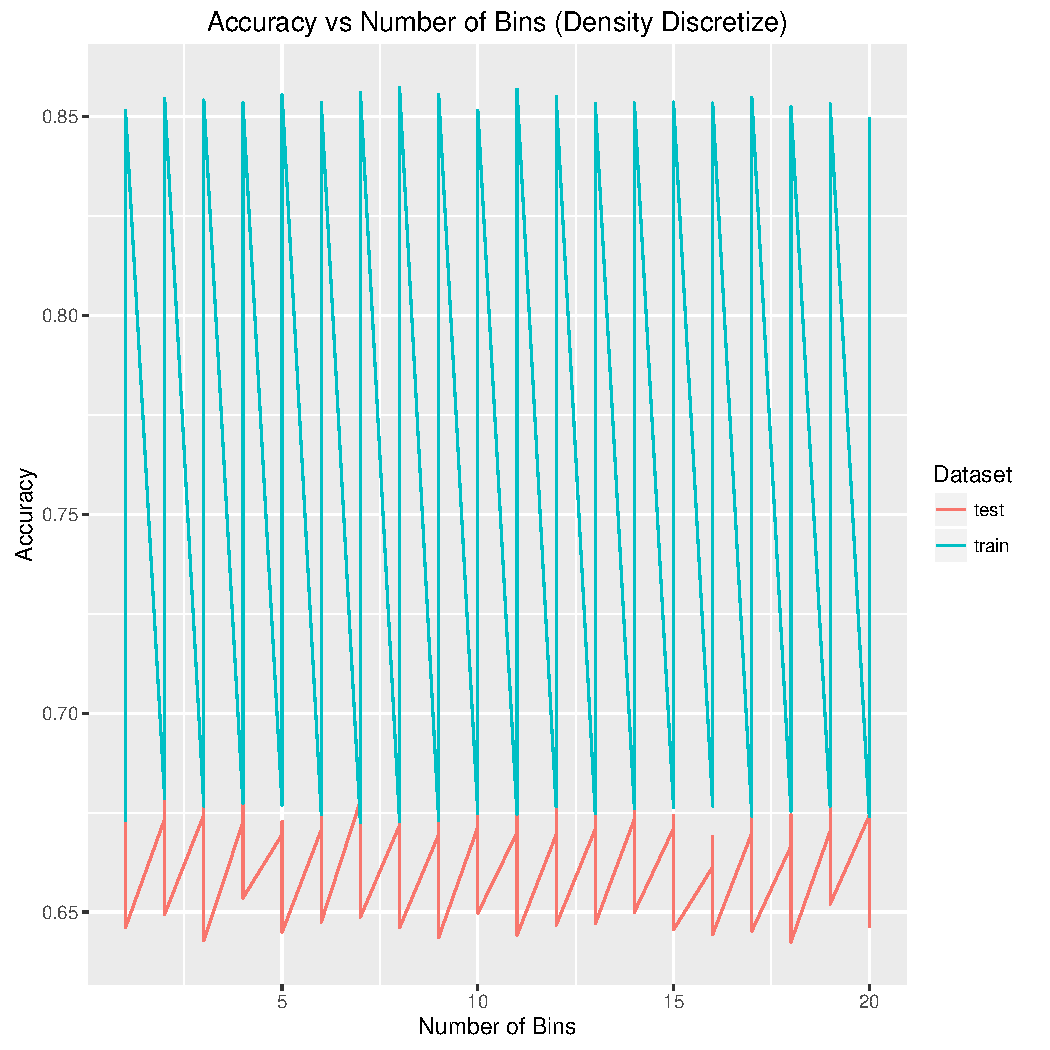
\includegraphics[width = 7cm]{6f.pdf}}
  \caption{Accuracy vs CF (Discretización)}
  \label{fig:discretize}
\end{figure*}




